\chapter{Approach and Implementation} % Main chapter title

\label{Chapter5} % For referencing the chapter elsewhere, use \ref{Chapter1} 

\lhead{Chapter 5. \emph{Approach and Evaluation}}

LINKED TEXT : LANGUAGES AND LOCALIZATION 
ID : AUTOGENERATED
XPATH AND CSS: STRUCTURE DEPENDENT
NAME: 
SPEED MATTERS TOO 
This section presents a brief overview of our approach including the  implementation blocks and evaluation for the robustness analysis of Selenium tests.

\section{Selenium Tests}
\label{sec:WritingTests}
\vspace{-2mm} The first phase of our approach involves writing Java-coded Selenium tests for the chosen reference versions of the AUT. Furthermore, in case of web applications having existing Selenium test-suites available for reasonable number of versions, we intend to leverage such tests for our analysis. Our approach treats the AUT as a black-box and executes system level tests using Selenium WebDriver framework. To improve the quality and maintainability of the tests, we aim to write modular Selenium tests adhering to the Page-Object pattern. To improve the stability of the tests, we intend to use attributes such as element-ID, name or CSS-selectors for detecting the GUI elements. In case of unavailability of these parameters, we may resort to detecting the elements using XPath or link text locators. 

During the development of the Selenium tests, we aim to locally execute and test them.  By employing these tests, we intend to cover the core application functionalities of the AUT. We intend to perform our experiment on 4-5 different web application subjects, preferably open-source. We intend to include the subjects from different domains along with sufficient number of major versions (3-5) and minor revisions/commits. We intend to include 3-5 applications in our set of experimental subjects, for which existing Selenium tests are available for usage. Moreover, to verify our approach during the initial stages we might include a relatively small scaled application subject.

\section{Generating Behavioral State Models}
\label{sec:BehavModels}

\vspace{-2mm}
Subsequently, in the second phase we plan to integrate these tests with \textit{WebMate} in order to identify the behavioral and GUI state level differences between the reference version and the subsequent versions of the AUT. In order to expedite this process, we aim to deploy multiple versions of the AUT in parallel, on a remote server such as a Linux based virtual machine. Figure  \ref{fig:deployment} depicts the overview of remote automatic deployment process; three versions of the AUT are running simultaneously against their individual database instances. The general test set-up to concurrently and independently execute tests across these versions and to extract behavioral state models is as depicted in figure \ref{fig:stateModelExtraction}.  \textit{WebMate} takes the Selenium test suite and the application’s base URL as input and executes the tests on different versions of the AUT to generate the behavioral state models. Afterwards we plan to detect the GUI level differences across these versions using \textit{WebMate}. During this phase, we provide \textit{WebMate} with the URLs for different application states as input. As output, \textit{WebMate} highlights the changed and/or missing GUI elements for different versions in comparison to the reference version of the AUT. Thereafter, we intend to map the behavioral state differences to GUI level differences to confirm whether changing active GUI elements (e.g. clickable fields, buttons) have manifested a changed application behavior.

\begin{figure}[h!]
\makeatletter 
\renewcommand{\thefigure}{\@arabic\c@figure}
\makeatother
    \centering
  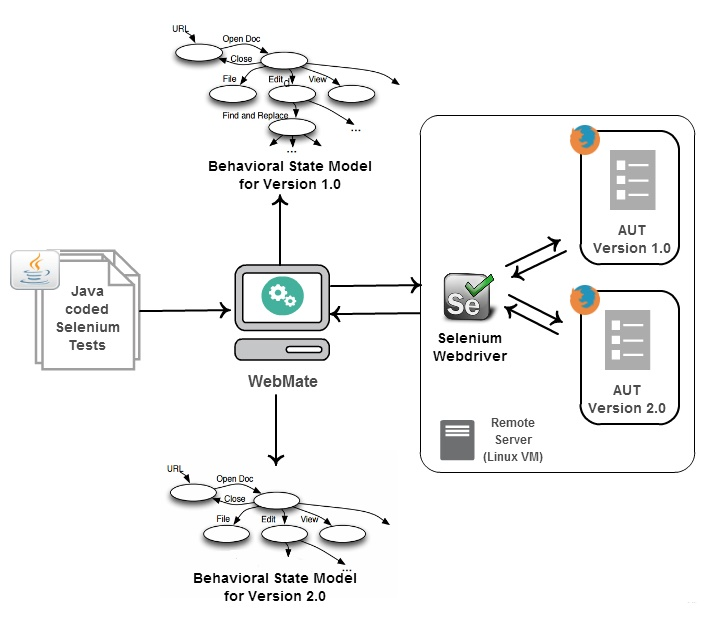
\includegraphics[width=5in,height=4in]{./Figures/WebMate_state_extraction}
  \caption{Extraction of behavioral state models using WebMate \cite{webmate}}
  \label{fig:stateModelExtraction} 
\end{figure}

\section{Measuring the Robustness Metric}
\label{sec:MeasureRobMetric}
\vspace{-2mm} To measure the robustness metric, we perform pair-wise equivalence check of the reference and test versions to assess whether same application states are covered. For cases where all the states are matched, robustness metric of given test-suite is 100\%. We propose to distribute the behavioral model generation and robustness measurement across the major and minor versions of the AUT, as mentioned in Section


\begin{center}
\begin{scriptsize}
\centering
\lstset{
  basicstyle=\ttfamily,
  columns=fullflexible,
  keepspaces=true,
%   frame=none,
}
% \verb|basicstyle=\ttfamily, columns=fullflexible, keepspaces=true|
  
\begin{lstlisting}[caption=Page-Objects design for \texttt{loginTest},label=code2]
actions : { 
[session-Id, get {url="http://application-under-test.com"}]
},
 actions : { 
[session-Id, findElement {using="id", value="username"}]
},
 actions : { 
[session-Id, sendKeysToElement {id="1", value=["uname"]}],
[session-Id, findElement {using="id", value="password"}]
},
 actions : { 
[session-Id, sendKeysToElement {id="2", value=["MOODLE_admin_121"]}],
[session-Id, findElement {using="link text", value="Login"}]
},
 actions : { 
[session-Id, clickElement {id="3"}]
}
\end{lstlisting}
\end{scriptsize} 
\end{center}